\section{Entwurfsmuster}

\begin{tcolorbox}[title=Entwurfsmuster]
    \textbf{Entwurfsmuster} sind wie Analyse- und Architekturmuster vorgefertigte Lösungsschablonen für verallgemeinerte Probleme des Entwurfs.\\

    \begin{itemize}
        \item \textbf{Beobachter (Observer)} - löst u.a.: eine Klasse soll die Möglichkeit haben, anderen Klassen Nachrichten zu senden;
         der Typ der empfangenden Klasse soll vorher nicht bekannt sein.
        \item \textbf{MVC (Model-View-Controller)} - löst u.a.: eine Anwendung verarbeitet Eingaben und reagiert (interaktiv) mit Ausgaben; die Verantwortlichkeiten werden sinnvoll verteilt.
        \item \textbf{Immutable} - löst u.a.: Änderungen der Inhalte der Referenzen wirken sich unerwünscht auf andere Objekte aus; sollte eine Änderung des internen Zustands benötigt sein, wird eine neue Instanz der Klasse mit den gewünschten Aktualisierungen erzeugt - das ursprüngliche Objekt bleibt so unverändert.
        \item \textbf{Iterator} - löst u.a.: Objekte sind in verschiedenen Datenstrukturen organisiert; die Struktur soll verborgen bleiben, damit sie für den sequentiellen Zugriff unerheblich ist; die Datenstruktur wird darüber leicht austauschbar.
        \item \textbf{Fassade } - löst u.a.: Klassen nutzen eine zusammengehörige Gruppe von zusammenarbeitenden Klassen;
        die Details der Gruppe sollen verborgen bleiben, damit einzelne Bestandteile leichter geändert oder ausgetauscht werden können
    \end{itemize}
\end{tcolorbox}

    \begin{figure}
        \centering
        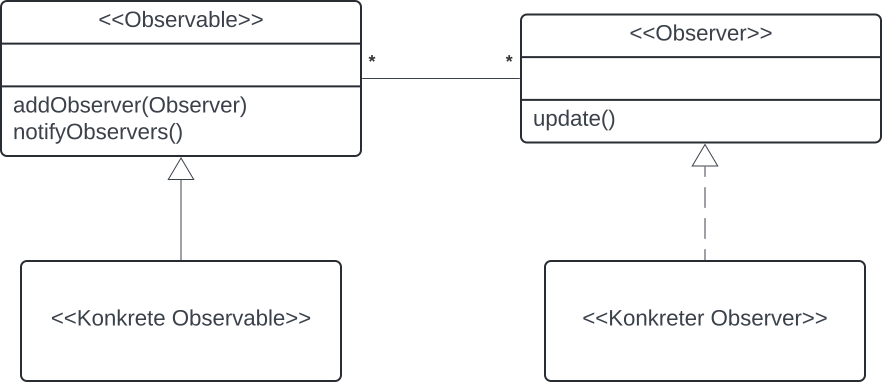
\includegraphics[scale=0.4]{part two/Objektorientierter Entwurf/img/observer}
        \caption{Klassendiagramm des Observer-Patterns (Quelle: eigene)}
        \label{fig:observer_cc}
    \end{figure}
    \begin{figure}
        \centering
        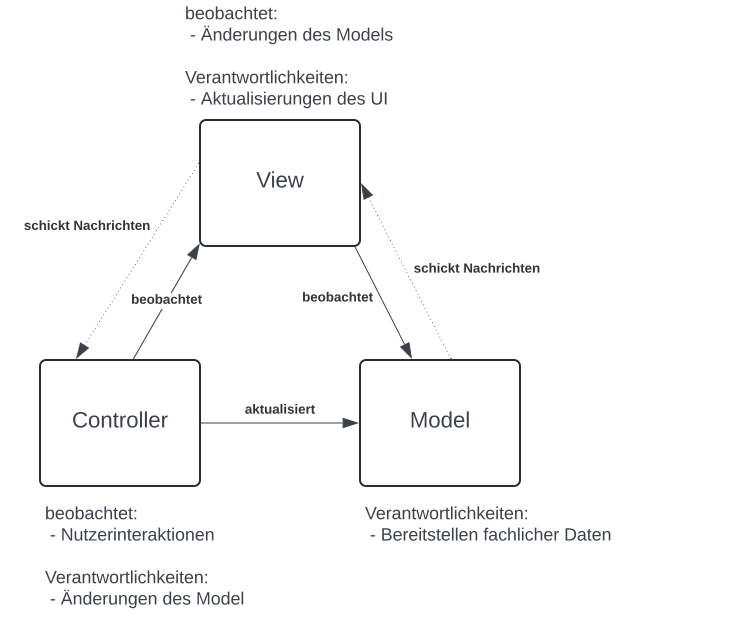
\includegraphics[scale=0.4]{part two/Objektorientierter Entwurf/img/mvc}
        \caption{Schematische Darstellung des MVC-Patterns mit seinen Verantwortlichkeiten (Quelle: eigene)}
        \label{fig:mvc_cc}
    \end{figure}
    \begin{figure}
        \centering
        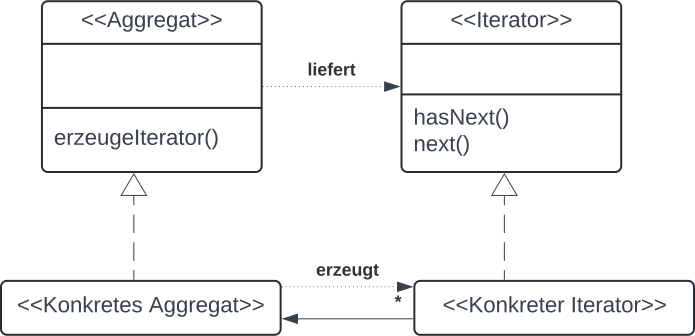
\includegraphics[scale=0.4]{part two/Objektorientierter Entwurf/img/iterator}
        \caption{Klassendiagramm des Iterator-Patterns (Quelle: in Anlehnung an~\cite[60, Abb. 3.9]{Wed09b})}
        \label{fig:iterator_cc}
    \end{figure}
\begin{figure}
    \centering
    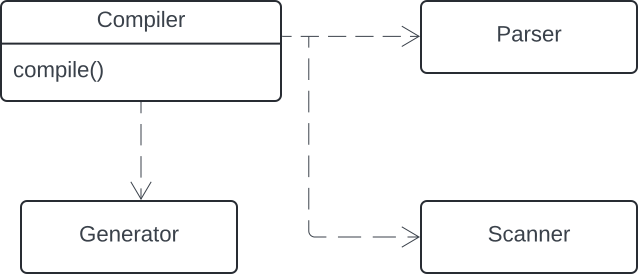
\includegraphics[scale=0.4]{chapters/Anhang/CheatSheets/SE2/img/fassade}
    \caption{Klassendiagramm einer Fassade (Quelle: in Anlehnung an \cite[186]{GHJV94})}
    \label{fig:fassade_cc}
\end{figure}
